\documentclass[oneside,a4paper,14pt]{extarticle}
\usepackage[T1,T2A]{fontenc}
\usepackage[
a4paper,
letterpaper,
top=2cm,
bottom=2cm,
left=2.5cm,
right=1.5cm
]{geometry}
\usepackage[utf8]{inputenc}
\usepackage[russian]{babel}
\usepackage{textcomp}
\usepackage{indentfirst}
\usepackage{listings}
\usepackage{xcolor}
\usepackage{enumitem}
\usepackage{graphicx}
\usepackage{mwe}
\usepackage{wrapfig}
\usepackage{caption}
\usepackage{amsmath}
\usepackage{amsfonts}
\usepackage{float}
\usepackage{amsthm}
\usepackage[all]{xy}
\usepackage[breaklinks]{hyperref}

\usepackage{titlesec}
\titleformat{\section}
{\normalsize\bfseries}
{\thesection} {1em}{}
\titleformat{\subsection}
{\normalsize\bfseries}
{\thesubsection} {1em}{}
\titleformat{\subsubsection}
{\normalsize\bfseries}
{\thesubsubsection} {1em}{}

\renewcommand\baselinestretch{1.33}
\normalsize
\setlength{\parindent}{1.25cm}

\lstset{
	language=SQL,
	basicstyle=\ttfamily\small,
	keywordstyle=\color{blue},
	commentstyle=\color{green!60!black},
	stringstyle=\color{red},
	numbers=left,
	numberstyle=\tiny\color{gray},
	frame=single,
	breaklines=true,
	showstringspaces=false,
	tabsize=4,
	inputencoding=utf8,
	extendedchars=true,
	literate={а}{{\selectfont\char224}}1 {б}{{\selectfont\char225}}1 {в}{{\selectfont\char226}}1 {г}{{\selectfont\char227}}1 {д}{{\selectfont\char228}}1 {е}{{\selectfont\char229}}1 {ж}{{\selectfont\char230}}1 {з}{{\selectfont\char231}}1 {и}{{\selectfont\char232}}1 {й}{{\selectfont\char233}}1 {к}{{\selectfont\char234}}1 {л}{{\selectfont\char235}}1 {м}{{\selectfont\char236}}1 {н}{{\selectfont\char237}}1 {о}{{\selectfont\char238}}1 {п}{{\selectfont\char239}}1 {р}{{\selectfont\char240}}1 {с}{{\selectfont\char241}}1 {т}{{\selectfont\char242}}1 {у}{{\selectfont\char243}}1 {ф}{{\selectfont\char244}}1 {х}{{\selectfont\char245}}1 {ц}{{\selectfont\char246}}1 {ч}{{\selectfont\char247}}1 {ш}{{\selectfont\char248}}1 {щ}{{\selectfont\char249}}1 {ъ}{{\selectfont\char250}}1 {ы}{{\selectfont\char251}}1 {ь}{{\selectfont\char252}}1 {э}{{\selectfont\char253}}1 {ю}{{\selectfont\char254}}1 {я}{{\selectfont\char255}}1 {А}{{\selectfont\char192}}1 {Б}{{\selectfont\char193}}1 {В}{{\selectfont\char194}}1 {Г}{{\selectfont\char195}}1 {Д}{{\selectfont\char196}}1 {Е}{{\selectfont\char197}}1 {Ж}{{\selectfont\char198}}1 {З}{{\selectfont\char199}}1 {И}{{\selectfont\char200}}1 {Й}{{\selectfont\char201}}1 {К}{{\selectfont\char202}}1 {Л}{{\selectfont\char203}}1 {М}{{\selectfont\char204}}1 {Н}{{\selectfont\char205}}1 {О}{{\selectfont\char206}}1 {П}{{\selectfont\char207}}1 {Р}{{\selectfont\char208}}1 {С}{{\selectfont\char209}}1 {Т}{{\selectfont\char210}}1 {У}{{\selectfont\char211}}1 {Ф}{{\selectfont\char212}}1 {Х}{{\selectfont\char213}}1 {Ц}{{\selectfont\char214}}1 {Ч}{{\selectfont\char215}}1 {Ш}{{\selectfont\char216}}1 {Щ}{{\selectfont\char217}}1 {Ъ}{{\selectfont\char218}}1 {Ы}{{\selectfont\char219}}1 {Ь}{{\selectfont\char220}}1 {Э}{{\selectfont\char221}}1 {Ю}{{\selectfont\char222}}1 {Я}{{\selectfont\char223}}1,
}

\begin{document}
	
	\newpage\thispagestyle{empty}
	\begin{center}
		МИНИСТЕРСТВО НАУКИ И ВЫСШЕГО ОБРАЗОВАНИЯ\\
		РОССИЙСКОЙ ФЕДЕРАЦИИ\\
		ФЕДЕРАЛЬНОЕ ГОСУДАРСТВЕННОЕ БЮДЖЕТНОЕ\\
		ОБРАЗОВАТЕЛЬНОЕ УЧРЕЖДЕНИЕ ВЫСШЕГО ОБРАЗОВАНИЯ\\
		<<ВЯТСКИЙ ГОСУДАРСТВЕННЫЙ УНИВЕРСИТЕТ>>\\
		Институт математики и информационных систем\\
		Факультет автоматики и вычислительной техники\\
		Кафедра электронных вычислительных машин
	\end{center}
	\vspace{20mm}
	\begin{center}
		Отчёт по лабораторной работе №1\\
		по дисциплине\\
		<<Базы данных>>\\
	\end{center}
	\vspace{48mm}
	\noindent
	Выполнил студент гр. ИВТб-1303-06-00 \hfill \rule[-0,5mm]{30mm}{0.15mm}\,/Шубин В. Ю./
	\newline
	Проверил преподаватель кафедры ЭВМ \hfill \rule[-0,5mm]{30mm}{0.15mm}\,/Клюкин В. Л./
	\vfill
	\begin{center}
		Киров\\
		2026
	\end{center}
	
	\newpage
	\thispagestyle{empty}
	
	\section*{Цель работы:} Познакомиться со схемами, пользователями и ролями в PostgreSQL, освоить основные варианты DDL-запросов, закрепить знания по проектированию структуры реляционной базы данных и создать рабочий материал для последующих лабораторных работ.
	
	\section*{Описание выбранной темы:} Выбранная тема для базы данных --- <<Видеоигры>>. База данных предназначена для учета студий-разработчиков, видеоигр, их жанров и отзывов пользователей. Структура спроектирована с учетом нормализации до третьей нормальной формы, прямые связи <<многие-ко-многим>> отсутствуют.
	
	\section*{Среда разработки:} PostgreSQL 18, pgAdmin 4, Windows 10.
	
	\newpage
	
	\section*{ER-диаграмма}
	ER-диаграмма разработанной структуры базы данных представлена на рисунке 1.
	
	\begin{figure}[H]
		\centering
		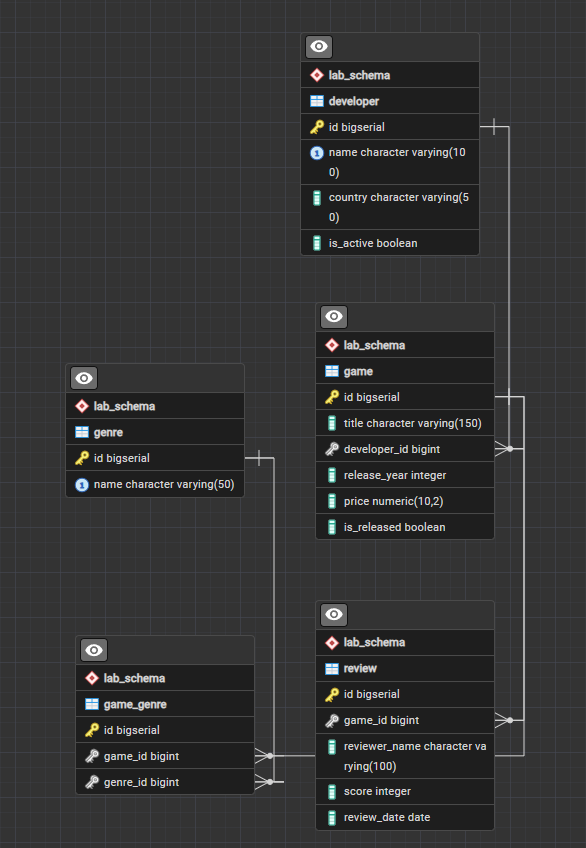
\includegraphics[width=10cm]{1.png}
		\caption{ER-диаграмма базы данных <<Видеоигры>>}
	\end{figure}
	
	\section*{Описание таблиц}
	\begin{enumerate}
		\item Таблица <<developer>> содержит информацию о студиях-разработчиках. Включает столбцы: <<id>> --- уникальный идентификатор, <<name>> --- название студии, <<country>> --- страна происхождения, <<is\_active>> --- флаг активности студии.
		\item Таблица <<genre>> содержит справочник жанров видеоигр. Включает столбцы: <<id>> --- уникальный идентификатор, <<name>> --- название жанра.
		\item Таблица <<game>> содержит основную информацию об играх. Включает столбцы: <<id>> --- уникальный идентификатор, <<title>> --- название игры, <<developer\_id>> --- внешний ключ к таблице разработчиков, <<release\_year>> --- год выхода, <<price>> --- цена игры, <<is\_released>> --- флаг релиза игры.
		\item Таблица <<game\_genre>> является промежуточной таблицей для реализации связи <<многие-ко-многим>> между играми и жанрами. Включает столбцы: <<id>> --- уникальный идентификатор связи, <<game\_id>> --- внешний ключ к таблице игр, <<genre\_id>> --- внешний ключ к таблице жанров.
		\item Таблица <<review>> содержит информацию об оценках и отзывах пользователей. Включает столбцы: <<id>> --- уникальный идентификатор, <<game\_id>> --- внешний ключ к таблице игр, <<reviewer\_name>> --- имя рецензента, <<score>> --- оценка от 1 до 10, <<review\_date>> --- дата написания отзыва.
	\end{enumerate}
	
	\section*{SQL-скрипт создания структуры БД}
	
	\begin{lstlisting}
		-- Создание таблицы разработчиков
		CREATE TABLE lab_schema.developer (
		id bigserial PRIMARY KEY,
		name varchar(100) NOT NULL UNIQUE,
		country varchar(50),
		is_active boolean NOT NULL DEFAULT true
		);
		
		-- Создание таблицы жанров
		CREATE TABLE lab_schema.genre (
		id bigserial PRIMARY KEY,
		name varchar(50) NOT NULL UNIQUE
		);
		
		-- Создание таблицы игр
		CREATE TABLE lab_schema.game (
		id bigserial PRIMARY KEY,
		title varchar(150) NOT NULL,
		developer_id bigint NOT NULL REFERENCES lab_schema.developer(id),
		release_year integer CHECK (release_year >= 1970 AND release_year <= 2030),
		price numeric(10, 2) CHECK (price >= 0),
		is_released boolean NOT NULL DEFAULT false
		);
		
		-- Создание промежуточной таблицы для связи игра-жанр
		CREATE TABLE lab_schema.game_genre (
		id bigserial PRIMARY KEY,
		game_id bigint NOT NULL REFERENCES lab_schema.game(id) ON DELETE CASCADE,
		genre_id bigint NOT NULL REFERENCES lab_schema.genre(id) ON DELETE CASCADE,
		UNIQUE (game_id, genre_id)
		);
		
		-- Создание таблицы отзывов
		CREATE TABLE lab_schema.review (
		id bigserial PRIMARY KEY,
		game_id bigint NOT NULL REFERENCES lab_schema.game(id) ON DELETE CASCADE,
		reviewer_name varchar(100) NOT NULL,
		score integer NOT NULL CHECK (score >= 1 AND score <= 10),
		review_date date NOT NULL DEFAULT CURRENT_DATE
		);
		
		-- Создание индексов для производительности
		CREATE INDEX idx_game_developer_id ON lab_schema.game(developer_id);
		CREATE INDEX idx_game_release_year ON lab_schema.game(release_year);
		CREATE INDEX idx_review_game_id ON lab_schema.review(game_id);
		CREATE INDEX idx_game_genre_game_id ON lab_schema.game_genre(game_id);
		
		-- Выдача прав пользователю lab_test
		GRANT ALL ON ALL TABLES IN SCHEMA lab_schema TO lab_test;
		GRANT ALL ON ALL SEQUENCES IN SCHEMA lab_schema TO lab_test;
	\end{lstlisting}
	
	\newpage
	\section*{Выводы} В ходе выполнения лабораторной работы была спроектирована и реализована структура реляционной базы данных на тему <<Видеоигры>>. Создан новый пользователь и пустая база данных. Разработана структура из 5 таблиц, удовлетворяющая третьей нормальной форме. Реализованы все необходимые DDL-запросы: первичные ключи, внешние ключи для ссылочной целостности, ограничения и индексы для оптимизации запросов. Пользователю выданы все необходимые права на работу с созданной схемой и объектами внутри неё. Рабочий материал для следующих лабораторных работ успешно создан.
	
\end{document}